\documentclass[tikz,border=2pt]{standalone}
\usepackage{amsmath,amssymb}
\usepackage{tikz}
\usetikzlibrary{arrows.meta}

\begin{document}
% Cramer's rule in the plane: b = x1 a1 + x2 a2, so the parallelogram spanned by b and a2 is
% the one spanned by a1 and a2 stretched by x1 (sheared, which keeps the area):
% det(b, a2) = x1 det(a1, a2).
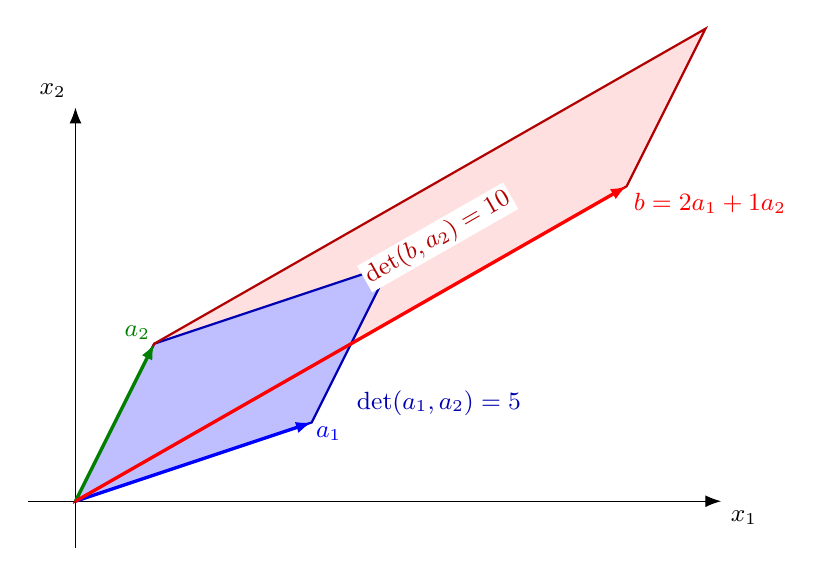
\begin{tikzpicture}[every node/.style={font=\small}, >={Latex[length=2mm]}]
	\draw[->] (-0.6,0) -- (8.2,0) node[below right] {$x_1$};
	\draw[->] (0,-0.6) -- (0,5.0) node[above left] {$x_2$};
	\fill[red!12] (0,0) -- (7,4) -- (8,6) -- (1,2) -- cycle;
	\fill[blue!25] (0,0) -- (3,1) -- (4,3) -- (1,2) -- cycle;
	\draw[blue!70!black, thick] (0,0) -- (3,1) -- (4,3) -- (1,2) -- cycle;
	\draw[red!70!black, thick] (0,0) -- (7,4) -- (8,6) -- (1,2) -- cycle;
	\draw[->, blue, very thick] (0,0) -- (3,1) node[below right, inner sep=1pt] {$a_1$};
	\draw[->, green!50!black, very thick] (0,0) -- (1,2) node[above left, inner sep=1pt] {$a_2$};
	\draw[->, red, very thick] (0,0) -- (7,4) node[below right, inner sep=2pt] {$b=2a_1+1a_2$};
	\node[blue!70!black, anchor=west] at (3.45,1.25) {$\det(a_1,a_2)=5$};
	\node[red!70!black, rotate=29.74, fill=white, inner sep=1pt] at (4.6,3.35) {$\det(b,a_2)=10$};
\end{tikzpicture}
\end{document}
